\title{Star Formation and Feedback in Stellar Clusters and Galaxies}

\author{PI: Mordecai-Mark Mac Low, American Museum of Natural History, New York.\\
        co-PIs: Andrew Emerick, Columbia University / AMNH, Joshua Wall, etc.}

\documentclass[11pt]{article}

\usepackage[letterpaper, margin=1in]{geometry}
\usepackage{amsmath}

\usepackage{natbib}
\usepackage{multirow}
\usepackage{multicol}
\usepackage{array}
\usepackage{graphicx}
\usepackage{epstopdf}
\epstopdfsetup{update}
\newcolumntype{L}{>{\centering\arraybackslash}m{2cm}}
\newcolumntype{R}{>{\centering\arraybackslash}m{1.25cm}}

\citestyle{aa}

\newcommand {\apj}{ApJ}
\newcommand {\aj}{AJ}
\newcommand {\apjs}{ApJS}
\newcommand {\apjl}{ApJL}
\newcommand {\mnras}{MNRAS}
\newcommand {\aap}{A\&A}
\newcommand {\aapr}{A\&ARv}
\newcommand {\araa}{ARA\&A}
\newcommand {\pasj}{PASJ}
\newcommand {\pasp}{PASP}
\newcommand {\bain}{Bulletin of the Astronomical Institutes of the Netherlands}
\newcommand {\fcp}{Fundamentals of Cosmic Physics}
\newcommand {\nat}{Nature}
\newcommand {\na}{New Astronomy}
\newcommand{\eg}{e.g.,}
\newcommand\rmxaa{Rev. Mex. Astron. Astrofis.} % Revista Mexicana de Astronomia y Astrofisica

\begin{document}
\maketitle

\section{Overview}

\section{Star Formation, Feedback, and Chemodynamics of Galaxies}

Recently, large scale, cosmological hydrodynamics simulations have been able to reproduce the observed properties of galaxies over a wide range of galaxy stellar masses and dark matter halo masses \citep[\eg][]{MUGS2010, MAGICC2013, Illustris1, Illustris2, OWLS, EAGLE, FIRE, APOSTLE, Latte}. These works have made strides in reconciling outstanding disagreements between predictions from $\Lambda$CDM cosmology and observations of nearby dwarf galaxies. Improvements in our understanding of baryonic physics, namely the feedback that self-regulates star formation in galaxies, has allowed these works to make strides in reconciling outstanding disagreements between predictions from $\Lambda$CDM cosmology and observations of nearby dwarf galaxies. However, due to computational constraints, feedback implementations are often phenomenological, tuned to reproduce observed galaxy properties. Clearly, given its role in galaxy evolution, a deeper understanding of feedback physics through high resolution, idealized simulations is necessary. We propose to conduct a sensitive test of the ability for various feedback processes to self-consistently reproduce dynamical, morphological, and chemical properties of dwarf galaxies simultaneously. We will conduct high resolution simulations of small dwarf galaxies, varying the underlying feedback physics, while tracing chemical abundances and stellar evolution on a star-by-star basis.

Historically, feedback physics in galaxies meant the injection of purely thermal energy in a localized region -- often with tricks to prevent rapid, unphysical overcooling of gas -- to model the effects of supernovae explosions. It has become clear feedback physics has to be modeled in much greater detail than just injecting thermal energy from supernovae. In addition to core collapse and Type Ia supernovae, we will include the effects of 1) energy injection from the winds of both AGB stars and massive stars, 2) radiation feedback (photoionization, photoheating, and radiation pressure) from massive stars followed through adaptive ray tracing, 3) a model for photoelectric heating of dust grains due to stellar radiation, and 4) cosmic rays (CR) injected at supernova sites, which provide a non-thermal additional pressure in the interstellar medium (ISM).

In general we have a fair understanding of the mean properties in the chemical evolution of galaxies, but models have difficulty in reproducing the observed scatter in both gas phase an stellar abundances. In particular, models of the chemical evolution of dwarf galaxies are often tuned to match the observed properties of a small number of observed galaxies. Self-consistently reproducing both the dynamic and chemical, or chemodynamics, properties of dwarf galaxies in hydrodynamics simulations remains a standing challenge for theoretical models. In addition, with one exception \citep{Few2012, Few2014}, all hydrodynamics simulations examining galactic chemodynamics have been implemented in smooth particle hydrodynamics (SPH) codes. Although historical problems with the SPH formalism have been improved substantially in recent years, they often still employ sub-grid mixing schemes to model mixing of spatially adjacent but chemically inhomogeneous gas \citep[\eg][]{ShenWadsleyStinson2010}. In part due to these methods, there are outstanding uncertainties in how much results depend on specific code implementations \citep{Revaz2016}. In addition, using star particles that represent clusters of stars becomes problematic at the high spatial and particle mass resolution needed for simulating low mass dwarf galaxies \citep{Revaz2016}. This motivates a new method for studying galactic chemical evolution in hydrodynamics simulations, including, for the first time, the full range of possible feedback physics while following individual stars. This is particularly exciting with recent or ongoing -- for example ANGST \citep{ANGST2009}, APOGEE \citep{APOGEE2010}, and GAIA -- and upcoming observational studies (e.g. APOGEE-2) that will obtain stellar abundance measurements in both our galaxy and nearby dwarfs, which will be the ideal comparison to our simulations of dwarf galaxies with individual, chemically tagged stars.

We provide a discussion of the feedback physics and associated models we propose to include in our simulations. We seek to understand how each of these processes individually and together affect galactic dynamical and chemical structure. 

\subsection{Discussion of Feedback Physics and Models}

To produce a controlled set of numerical experiments on the effect of various feedback physics on galaxy evolution, we will initialize our galaxy as a semi-spherical gas cloud embedded in a dark matter background potential, and simulate it through collapse until just before first star formation. This collapsed gas cloud will serve as the initial conditions from which we will vary the underlying feedback physics. Differences in the subsequent evolution will be analyzed to understand the role of each feedback mechanism. 

The following physics will identical in each simulation: 1) gas self-gravity to capture the collapse and concomitant star formation in dense regions, 2) a 9 species non-equillibrium chemistry solver, following electrons and H, He, and H$_{2}$ and their ionization states \citep{Anninos1997, Abel1997}, 3) associated heating / cooling as followed in the \texttt{Grackle} library (Smith et. al. in prep), including heating from a metagalactic UV background \citep{HM2012} and tabulated metal line cooling from \texttt{Cloudy} \citep{Cloudy2013}, 4) approximate H and He gas self-shielding of the UV background \citep{Rahmati2013}, 5) a metagalactic Lyman-Werner (LW) flux from \cite{HM2012} to properly model H$_{2}$ dissociation, as well as an optically thin LW flux from each of our stars to account for local LW fluctuations in the galaxy, and 6) a collisionless N-body solver to evolve the dynamics of the formed star particles. In every simulation, we form stars from dense gas in the highest refined region (1 pc) following a stochastic star formation scheme from \cite{Goldbaum2015, Goldbaum2016}, modified to sample individual stellar masses from an input IMF \citep{Salpeter1955}. Each star is chemically tagged by the local gas abundances, and assigned stellar properties from a grid of stellar evolution tracks \citep{Bressan2012}, which ultimately govern the radiative properties of the stars (if radiation feedback is used), the stellar wind velocity, and the star's lifetime.

Since they are the sources of chemical enrichment in galaxies, our key observational discriminator between feedback mechanisms, supernovae and stellar wind feedback will be treated uniformly in all simulations. Stellar yields for both winds and supernovae are taken from the NuGrid data set \citep[][, Ritter et. al. in prep]{Pignatari2016}, a self-consistent model of stellar yields over a well sampled range of stellar masses ($M_{*} \in [1,25]~M_{\odot}$) and metallicities ($Z\in [10^{-4},0.2]$). We model stellar winds from massive stars ($M > 8~M_{\odot}$) using a constant mass loss rate over their lifetimes, while low mass stars ($M < 8~M_{\odot}$) remain quiescent until a final AGB phase wind emitted near the very end of their lifetimes. Stellar properties, including lifetimes, AGB phase star times, radius, surface gravity, and effective temperature are obtained via interpolation over the \texttt{PARSEC} grid of stellar evolution tracks \citep{Bressan2012}\footnote{Stellar radius, surface, gravity, and effective temperature are used only for determining radiation properties of our stars, and play no direct role in our simulations}. Stars below 8 M$_{\odot}$ are tracked after their death as white dwarf particles, assigning white dwarf masses from the observed initial-to-final-mass distribution \citep{Salaris2009}. Following \citep{Cote2015}, we use an observationally motivated delay time distribution model \citep[\eg][]{Maoz2014} to assign to each white dwarf a time when they will explode as a Type Ia supernova.\footnote{We note that only a few percent of white dwarfs should explode as Type Ia in a Hubble time \citep{Maoz2014}; our model takes this into account in assigning explosion times, with a large majority never exploding.} We adopt Type Ia supernova yields from \cite{Thielemann1986}.

Accounting for the effects of CRs in galaxy scale simulations has only been possible recently, yet has been shown to likely be a very important source of additional feedback in galaxies \citep[\eg][]{SalemBryan2014, SalemBryanHummels, SalemBryanCorlies, GirichidisCR, Pakmor2016, Simpson2016}. The role of CRs in low mass dwarf galaxies is still uncertain, though has been investigated recently in more massive dwarfs than those considered in this proposal \citep{Chen2016}. The implementation of CR feedback in \texttt{Enzo} \citep{SalemBryan2014} assumes both isotropic diffusion and ignores energy losses from interactions with an ordered magnetic field. Isotropic diffusion in very low mass dwarf galaxies may not be a poor assumption, as their lack of obvious disk structure may indicate that they lack the ability to create a global, ordered magnetic field that causes substantial anisotropies in CR behavior. We inject CR energy during supernova explosions at 10\% of the total energy injected, reducing the subsequent thermal / kinetic energy injection accordingly. CRs in our simulations are allowed to diffuse isotropically as controlled by a diffusion coefficient, and interacting with the hydrodynamics through an additional, non-thermal pressure term.

Radiation from massive stars provides a substantial additional source of feedback in galaxies \citep[\eg][]{Agertz2013}. Including radiative feedback has been shown XXXX (sources). Radiation fluxes for each of our stars are computed using the \texttt{OSTAR2002} grid of stellar atmosphere models \citep{Lanz2003}; for stars with effective temperatures below those sampled on the \texttt{OSTAR2002} grid, we compute radiation rates assuming a black body spectrum, scaled to be consistent with the \texttt{OSTAR2002} models. In this proposal, we include radiative feedback in two distinct forms: 1) H and He ionizing radiation, dominated from massive stars, and 2) local FUV flux from all stars that contributes to photoelectric heating within the ISM. Separating these physics will allow us to directly address recent disagreement in the role of photoelectric heating in dwarf galaxies \citep{Hu2016, Forbes2016}. We use \texttt{Enzo}'s radiative transfer capabilities \citep{Wise2012a,WiseAbel2012,Wise2014} to track ionizing radiation directly, coupling the ionizing / heating rates to the \texttt{Grackle} chemistry solver, and accounting directly for effects of H radiation pressure. We assume the FUV radiation to be everywhere optically thin, using a photoelectric heating rate model from \cite{BakesTielens1994} and \cite{Wolfire2003} that scales with local density, temperature, and metallicity.

\begin{figure}
\centering
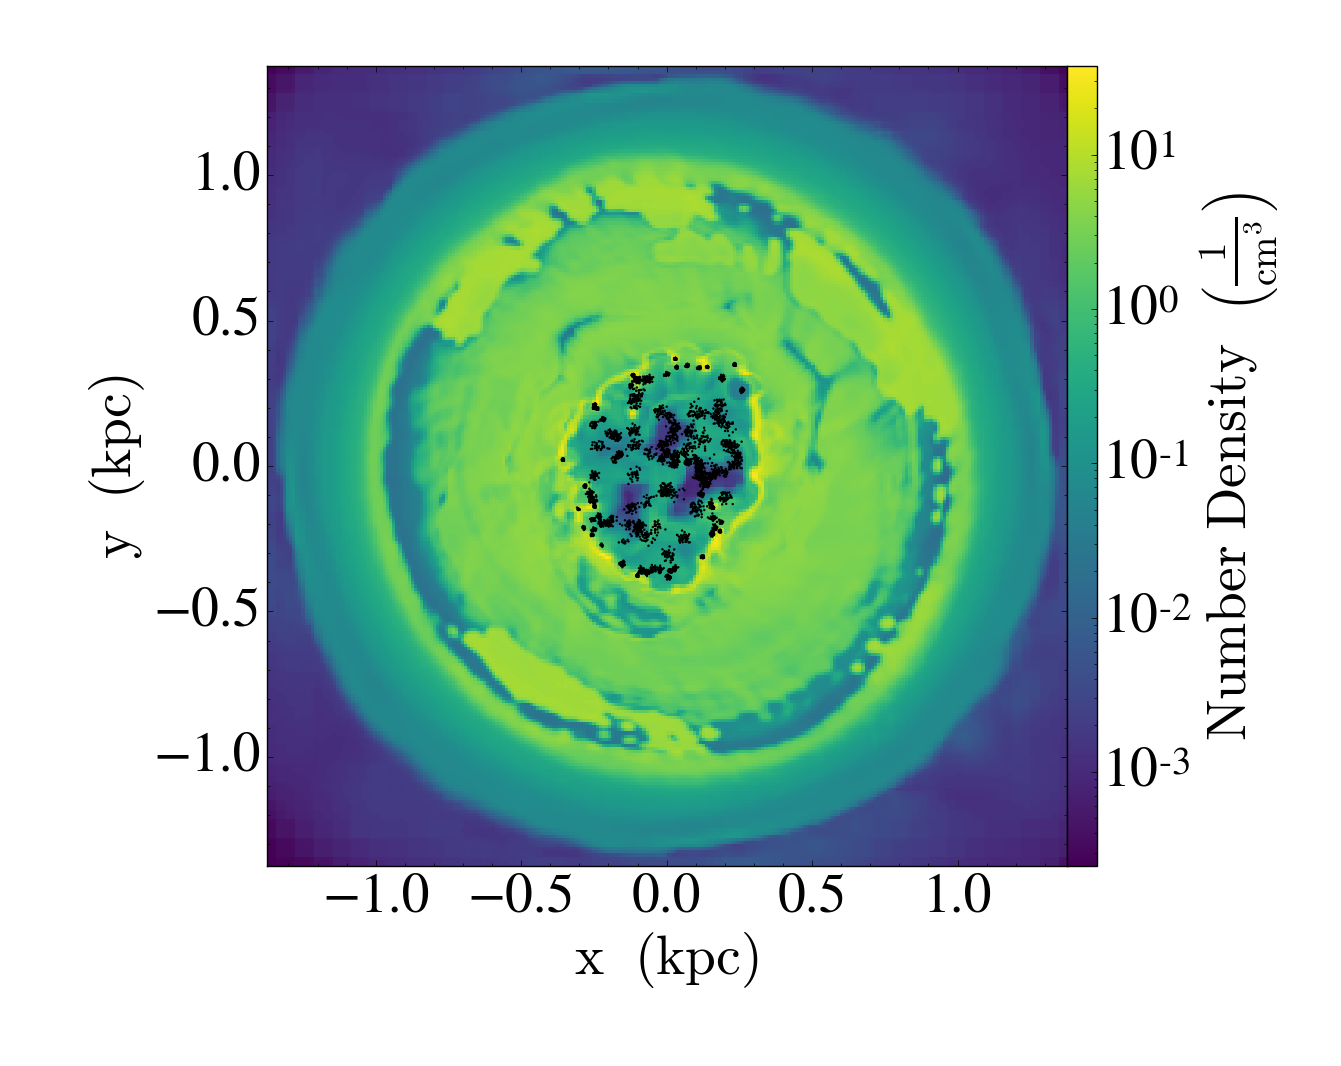
\includegraphics[width=0.45\linewidth]{number_density_slice}
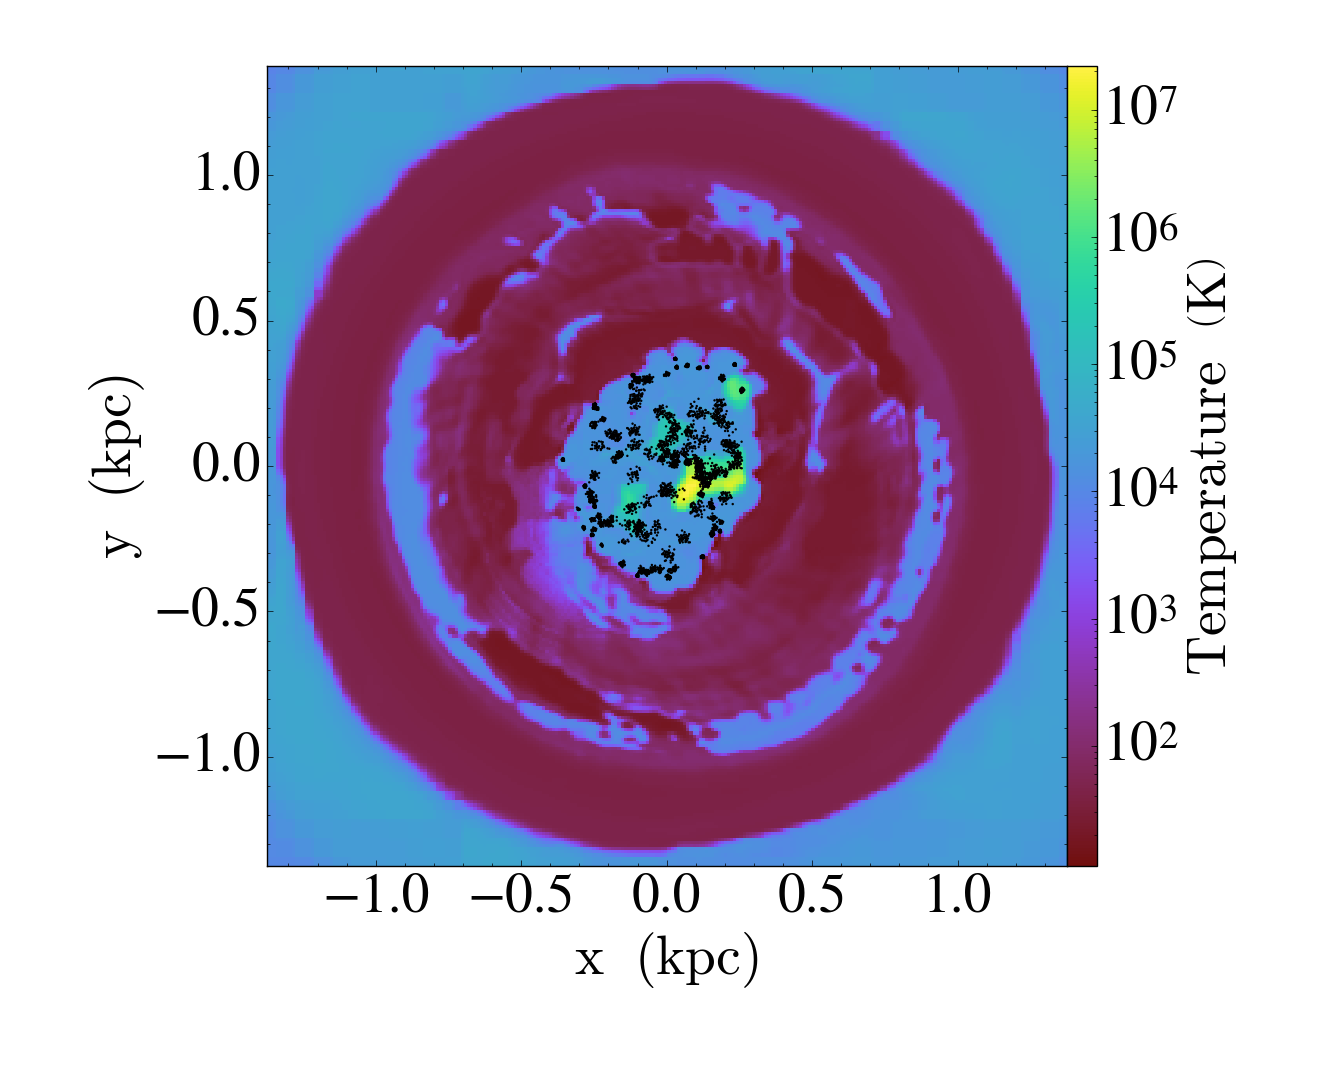
\includegraphics[width=0.45\linewidth]{temperature_slice}
\vspace{0.1cm}
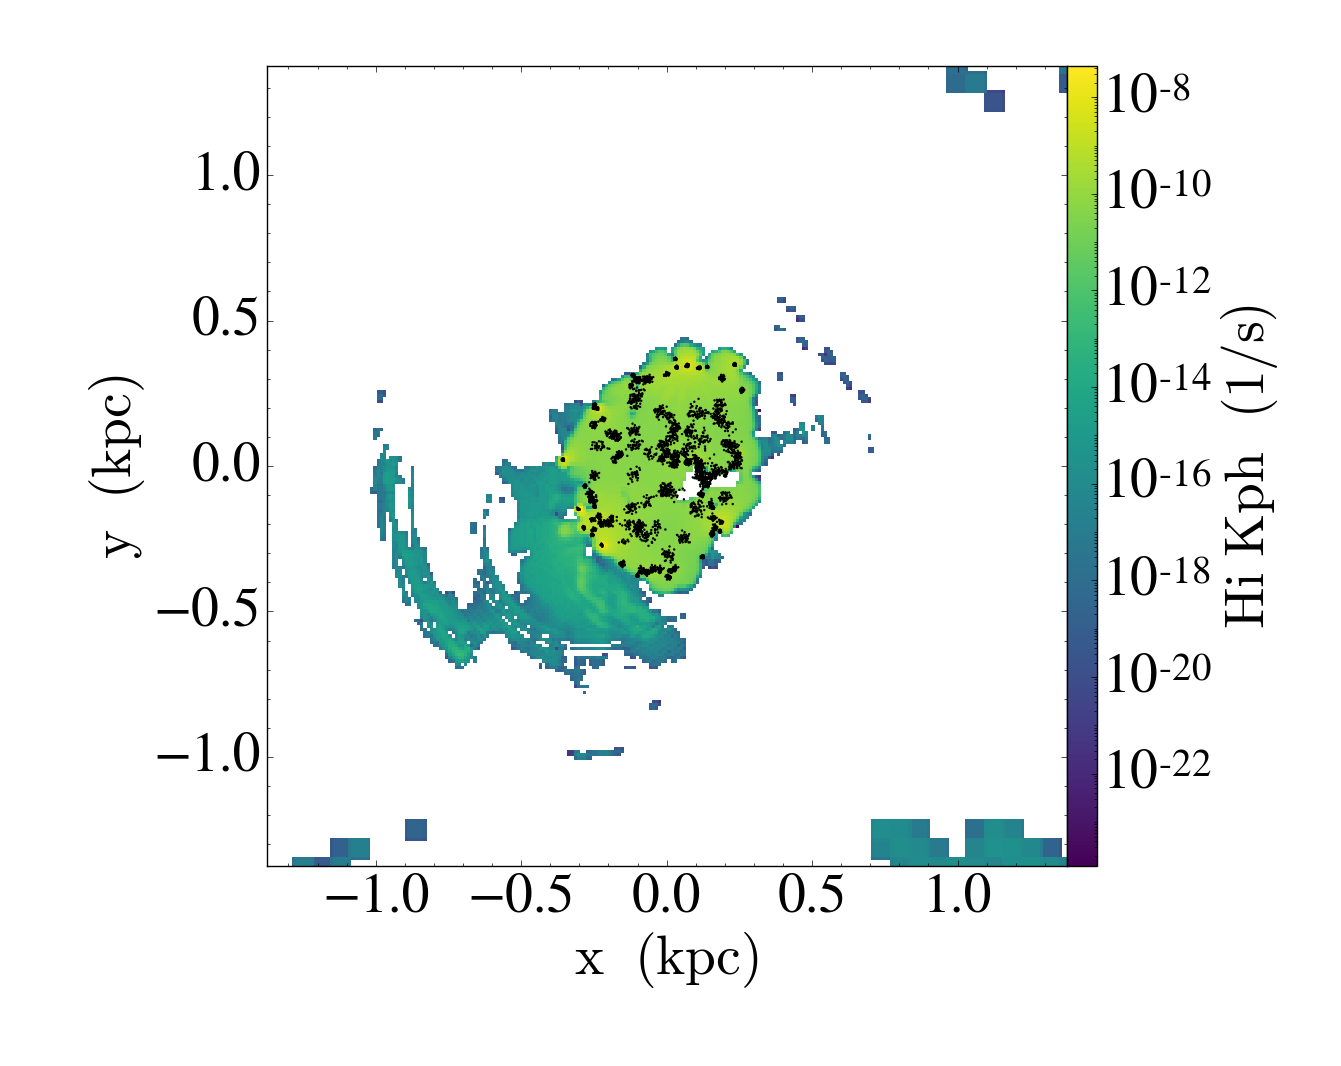
\includegraphics[width=0.45\linewidth]{hi_radiation_slice}
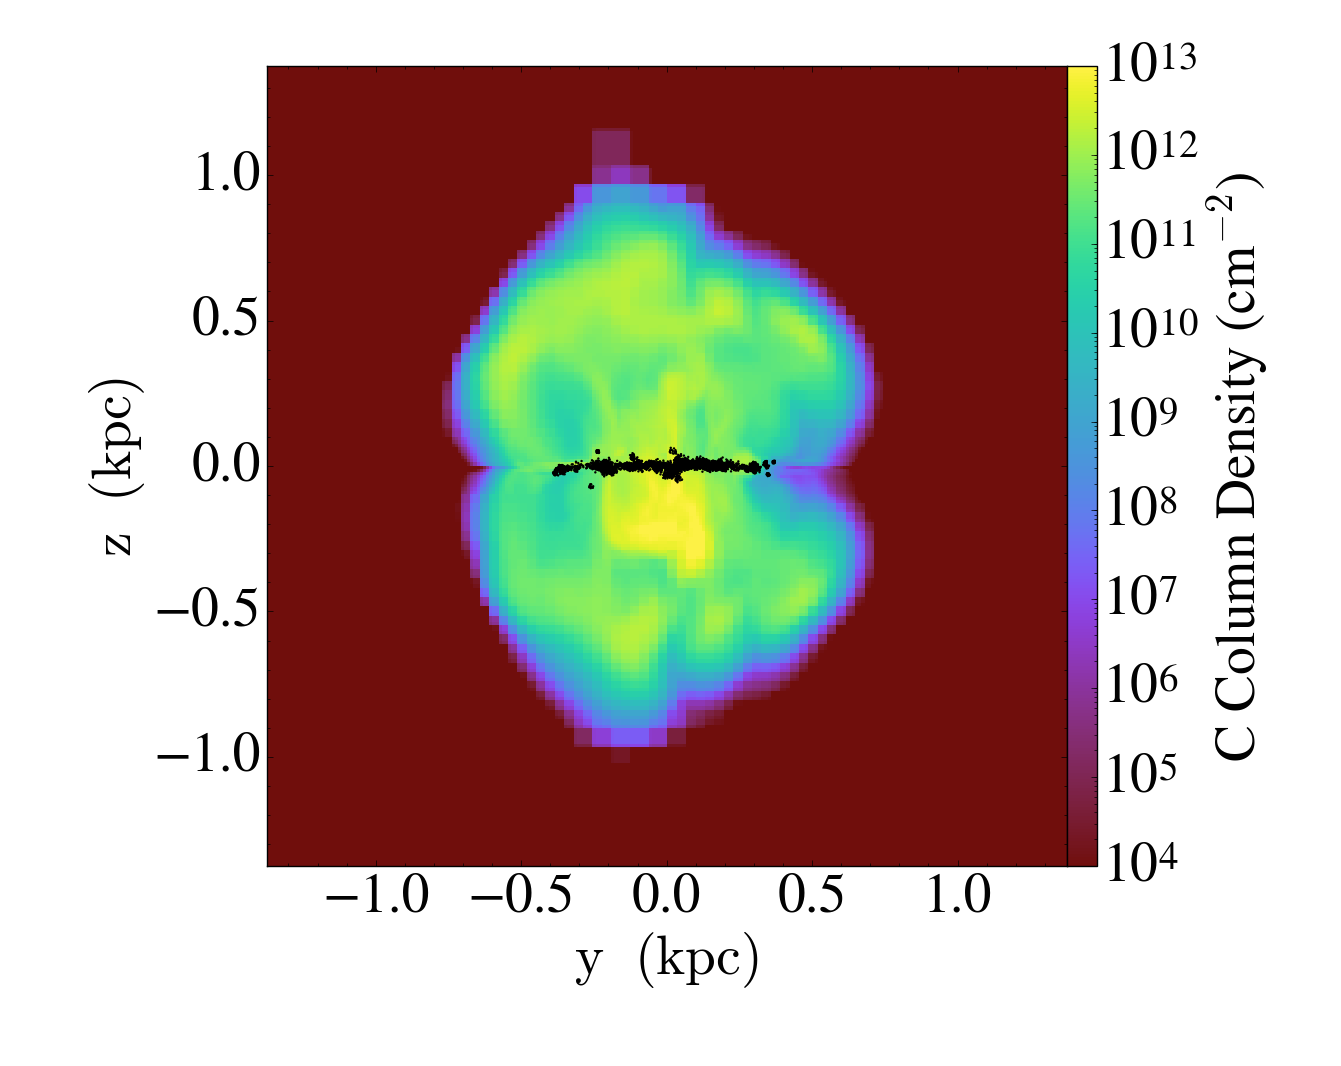
\includegraphics[width=0.45\linewidth]{c_projection}
\caption{Example images from a proof of concept test of our dwarf galaxy model at low resolution (8 pc). Shown here are face-on slices of number density (top left), temperature (top right), and HI ionizing radiation (bottom left), along with an edge-on projection of total Carbon column density, illustrating yields ejected in metal enriched winds. This test was run with supernovae, stellar winds, radiative transfer, and photoelectric heating. Each black dot in the images is a star particle, which are often too clustered to distinguish between individual particles in these zoomed-out images. These images show the simulation $\sim$60 Myr after star formation, at which point there are 4324 star particles with total mass $1.2\times10^5$ M$_{\odot}$. 173 of these particles are ionizing sources.}
\label{fig:levels}
\end{figure}

\subsection{Computational Methods}

Our dwarf galaxy simulations will be carried out using \textsc{Enzo}\footnote{www.enzo-project.org}, an adaptive mesh refinement (AMR) hydrodynamics and N-body code. \textsc{Enzo} is an entirely open-source code that is undergoing active development by many researchers across several institutions; its most recent stable release is version 2.5. This project involves a substantial amount of additional code development built on top of the development version of \textsc{Enzo} (version 2.X), and is also publicly available at www.bitbucket.org/aemerick/enzo-emerick. \textsc{Enzo} has been well tested and extensively used in a variety of applications, from XXX (Cite) to XXX (cite), including isolated galaxy simulations, as we propose here \citep[\eg][]{Goldbaum2015, Goldbaum2016, Forbes2016}. We outline the methods employed in \textsc{Enzo} as relevant to our proposal; a detailed description of these methods can be found in the \textsc{Enzo} method paper \citep{Enzo2014}. 

Each dwarf galaxy is centered on a uniform $128^3$ cell mesh with physical dimensions of $16.384^3$ kpc, corresponding to a root grid resolution of 128 pc. Additional levels of refinement are applied to regions surpassing a chosen density contrast and with the requirement that the Jeans length be resolved by 16 cells at all times \citep{Truelove}. Each level increases the resolution by a factor of 2, allowing us to achieve 1 pc resolution with a total of 7 levels of refinement. In addition, we force refinement around all star particles, such that feedback injection is always resolved at the maximum refinement level. \textsc{Enzo} employs adaptive time steps, evolving each refinement level independently with timestep size set by the Courant-Friedrichs-Levy condition for numerical stability. The exact size of each step is thus dependent on the local sound speed and gas velocity. Since supernova can heat the ISM to temperatures on order of 10$^{6-7}$ K, and stellar winds have velocities on order of 10$^{3}$ km s$^{-1}$, we expect typical timesteps on order of 10$^{2-3}$ years on our most refined level.

We couple \textsc{ENZO} to the open-source \texttt{Grackle} chemistry and heating/cooling library, which operates cell-by-cell on each grid. \texttt{Grackle} sub-cycles through a non-equillibrium chemistry solver following methods first used in \cite{Anninos1997} and \cite{Abel1997} that solves for the correct densities and ionization states of each species (), while accounting for radiative cooling and heating from external radiation fields.

CR's are traced using the two-fluid approximation as implemented in \cite{SalemBryan2014}. This secondary fluid is coupled to the hydrodynamics through a pressure term, acting as an additional, non-thermal pressure source in our simulations. CR diffusion is computed with an explicit finite difference scheme, which places an additional constraint on the size of each timestep, addressed by subcycling over the CR evolution. The CR timestep scales with the square of the cell size and is inversely proportional to the adopted diffusion coefficient. For a diffusion coefficient of $3\times10^{28}$~cm$^{2}$~s$^{-1}$, this corresponds to a reduction of a factor of $\sim$10 in our maximum time step size over runs without CR's.

We use the direct ray tracing from \cite{WiseAbel2011} in \texttt{Enzo} to directly follow the HI and HeI ionizing radiation from massive stars. This is an adaptive ray tracing method that splits rays using mapping to / from a \texttt{HEALPix} grid. These methods are well tested and have been used previously in cosmological simulations of reionization in the early Universe \citep{Wise2012a, WiseAbel2012,Wise2014, Kim2013a, Kim2013b}. These methods have been demonstrated to scale to $\mathcal{O}(10^{3})$ for large domains (up to $\sim 10^9$ cells) and many sources ($\sim10^{4}$). Although we only expect on order of several hundred sources at any one time in our simulations, direct ray tracing still incurs a significant additional expense. However, it is required in order to accurately capture radiation feedback in galaxies. We mitigate the additional cost somewhat by allowing for merging of rays that have traveled far from their sources (i.e. well outside or dwarf galaxy), and a reduced speed of light approximation at $0.1\rm{c}$.

\section{Justification of Resources}

We request a total of XXX million SU's and XX TB of storage space, as explained below for each of our projects.

\subsection{Feedback and Chemodynamics in Galaxies}

Our primary objective is to test the role various feedback physics play in the structural, dynamical, and chemical evolution of low mass dwarf galaxies. These will ultimately be tied to observational distinctions in the star formation history of our galaxies, distribution and retention of chemical ejecta in our galaxies, and the spatial distribution and abundances of the individual star particles. This is a pivotal test of whether or not widely used, approximate feedback methods are consistent with a detailed implementation. The computational cost of these methods, and our requirement for high resolution to well resolve the energy injection scales are the dominant source the large number of SU's we require. This is justifiable as these simulations will be vital for understanding of feedback physics, dwarf galaxy chemical and dynamical evolution, and can be extended to producing improved approximate feedback methods in larger scale simulations. We outline the cost and variations for each of our individual runs, as presented in Table~\ref{table:SU}, below.

\begin{table}

 \centering
 \footnotesize

 \begin{tabular}{| R | R | R | R | R | r | r | r | R |}
 \hline
 \multicolumn{1}{|m{1.5cm}|}{Model Number} & \multicolumn{1}{m{1.2cm}|}{SN and Winds} & \multicolumn{1}{m{1.75cm}|}{Ionizing Radiation} & \multicolumn{1}{m{0.5cm}|}{Cosmic Rays} & \multicolumn{1}{m{1.25cm}|}{PE Heating} & Resolution (pc) & 10$^{3}$ SU/Myr & Time (Gyr) & \multicolumn{1}{m{1.0cm}|}{Total SU (10$^{6}$)} \\
 \hline

  1 & Y  & N & N & N & 1.0 & 0.82 & 1.0 & 0.5 \\
  2 & Y* & N & N & N & 1.0 & 0.7  & 1.0 & 0.4 \\
  3 & Y  & Y & N & N & 1.0 & 2.0  & 1.0 & 3.0 \\
  4 & Y  & N & Y & N & 1.0 & 1.2  & 1.0 & 2.0 \\
  5 & Y  & N & N & Y & 1.0 & 0.9  & 1.0 & 0.5 \\
  6 & Y  & Y & N & Y & 1.0 & 2.0  & 1.0 & 3.0 \\
  7 & Y  & Y & Y & Y & 1.0 & 2.4  & 1.0 & 5.0 \\
  8 & Y  & Y & Y & Y & 0.5 & 16.0 & 0.1 & 4.0  \\  
  \hline
  Total & - & - & - & - & - & - & - & 18.4  \\
 \hline
 \end{tabular}

 \caption{Shown is a list of our planned simulations and the various feedback physics included in each. Stellar winds and supernovae are consistent in each case, except in model 2, where we ignore stellar wind energy injection (see text). Each simulation has a maximum spatial resolution of 1 pc with the exception of model 8, which will be run for a shorter time at 0.5 pc resolution.}
   \label{table:SU}
\end{table}

\begin{table}
 \centering
 \footnotesize
 \begin{tabular}{| R | R | R | R | R | R | R  | R }
 \hline
 \multicolumn{1}{|m{1.5cm}|}{Model Number} & \multicolumn{1}{m{1cm}|}{Number of Fields} & \multicolumn{1}{m{2.25 cm}|}{Number of Particle Fields} & \multicolumn{1}{m{2.0cm}|}{Memory Per Output (Gb)} & \multicolumn{1}{m{1.75 cm}|}{Short / Long Term Cadence (Myr)} & \multicolumn{1}{m{1.5cm}|}{Short Term Storage (TB)} & \multicolumn{1}{m{1.5cm}|}{Long Term Storage (TB)} \\
 \hline

  1 & 31 & 23 & 2.7 &  2.5 / 10 & 1.08 & 0.27  \\
  2 & 31 & 23 & 2.7 &  2.5 / 10 & 1.08 & 0.27  \\  
  3 & 38 & 23 & 3.2 &  2.5 / 10 & 1.28 & 0.32  \\
  4 & 32 & 23 & 2.7 &  2.5 / 10 & 1.08 & 0.27  \\
  5 & 33 & 23 & 2.8 &  2.5 / 10 & 1.12 & 0.28  \\
  6 & 40 & 23 & 3.4 &  2.5 / 10 & 1.36 & 0.34  \\
  7 & 41 & 23 & 3.5 &  2.5 / 10 & 1.40 & 0.35  \\
  8 & 41 & 23 & 33  &  0.5 / 5  & 6.60  & 3.3  \\  
  \hline
  TOTAL & - & - & - & - & 15.0 & 5.40 \\
 \hline
 \end{tabular}
 \caption{The estimated short and long term memory storage requirements for each of our simulations, and the total storage requested for this portion of our project. Each of the above grid and particle fields are stored as a 64 bit float. The above calculations are made assuming a typical grid cell count of $\sim 10^{7}$ and particle count of $\sim 10^{6}$. For our short, high resolution simulation (model 8) we expect on order of $\sim 10^{8}$ grid cells. Our 1 Gyr runs (models 1 - 7) will have a total of 400 short term and 100 long term outputs, and our high resolution will have 200 short term and 20 long term outputs.}
\end{table}

We trace a total of ten metal abundances in each simulation, restricting ourselves to those most readily constrained by observations \citep[see][and references therein]{Tolstoy2009}: C, N, O, Mg, Si, S, Fe, Ni, Y, and Eu. Stellar winds and supernovae are treated consistently in all models, with the exception of model 2. In model 2 we test the global importance of stellar wind feedback, leaving metal pollution by stellar winds on, but ignoring their energy injection into the ISM. Each subsequent simulation, models 3 through 6, varies the combination of feedback physics included, which we separate into ionizing radiation (radiative transfer), CRs, and photoelectric heating. Model 7 combines all of these mechanisms in a single simulation. Finally, we perform a resolution test at higher resolution (model 8) and lower resolution (model 9) to better understand the limitations even 1 pc resolution places on these physics. As indicated in Table~\ref{table:SU}, the additional estimated computational expense of a 0.5 parsec resolution simulation restricts us to a reduced simulation time of 100 Myr. For this reason, we will use one of the model 7 outputs at 500 Myr as the initial conditions of model 8, to ensure all feedback mechanisms are active for a more faithful resolution study. For consistency, we will simulate the low resolution model (model 9) over the same period of time, but for a small fraction of the cost.

The SU / Myr cost of each simulation is controlled by the total number of grid cells, size of each timestep, and whether or not radiative transfer is included. We estimate that the high velocity stellar winds (10$^{2-3}$ km s$^{-1}$) and hot gas from supernovae and shocks (10$^{6-7}$ K) will restrict the the maximum refinement level to timesteps on order of a few hundred to few thousand years. Based upon our initial tests at our fiducial resolution, we estimate the simulations will contain approximately 2$\times$10$^{7}$ cells, a majority of which would be on the highest refinement level. Our scaling tests show \textsc{Enzo} operates at roughly 10$^{4}$ cell updates per second per processor. We expect to run on 256 processors for a majority of the simulation time, giving a total cell update rate of roughly 2.5$\times 10^{6}$ cells per second across all processors. For a timestep of 500 years, this equates to 4.44 wall hours per Myr, or for 256 processors, or about 1.1$\times 10^{3}$ SU / Myr, and roughly a million hours per Gyr. These numbers are reflected in model 1 in Table~\ref{table:SU}. The additional cost of PE heating is likely insignificant, and may actually be cheaper as the additional heating may prevent additional star formation. The cost of radiative transfer is hard to estimate as it is tied directly to the number and concentration of radiation sources. However, after the first couple Myr of our simulations, we expect on order of 10$^{5-6}$ star particles. Based on our IMF, we expect only (roughly) a few to several hundred radiating stars ($M > 8 M_{\odot}$) at any one point in time. We estimate the additional cost incurred by these sources will be about a factor of 4 over model 1.

We plan to run each simulation for at least 1 Gyr, outputting data dumps every 2.5 Myr. We estimate that this cadence is necessary to provide access to on order of 1-3 restart dumps within a single job submission. Rapid analysis of this high cadence will allow us to understand the short timescale variance of dwarf galaxy chemodynamics; these will also be used to make high time resolution movies of our simulation set. Each output contains all of the information about the simulation at a single time. The memory required for each dump varies depending on the physics used as follows. Each simulation dump will contain 11 fields associated with the hydrodynamics and 20 fields associated with the primordial chemistry and metal abundances tracers, for a base total of 31. Radiative transfer (ionizing radiation) simulations will contain an additional 7, while photoelectric heating and Lyman Werner adds an additional 2. CRs only add a single additional field, for a total of 41 baryon fields in our full physics simulations. Each particle keeps track of 23 properties, 13 of which are abundances (metallicity, H, He, and metal tracers), while the rest include position (3), velocity (3), current mass, birth mass, lifetime, and formation time. Given this, our output cadence, the expected $2 \times 10^{7}$ cells, and the expected 10$^{5-6}$ star particles, we present our estimated memory storage requirements in Table~\ref{table:memory}.

\section{Project team qualifications}

\textbf{PI: Mordecai-Mark Mac Low}...........

\textbf{co-PI: Andrew Emerick} is a PhD student at Columbia University advised by both PI Mac Low and with collaborator Greg Bryan. Emerick is the developer of the new star formation and feedback models to be used in the star formation and feedback simulations of isolated dwarf galaxies in \textsc{Enzo}. He drafted this portion of the proposal, as it will comprise the bulk of his thesis research. Previously he has published research working with both \textsc{ENZO}, making synthetic absorption observations of gas in galaxy clusters \citep{Emerick2015}, and \textsc{FLASH}, studying gas stripping and feedback in low mass dwarf galaxy satellites \citep{Emerick2016}.

\textbf{co-PI: Joshua Wall}.......

\textbf{Collaborator: Greg Bryan} is a professor at Columbia University and {\bf title} at the Center for Computational Astrophysics at the Flatiron Institute. Bryan is the creator of the \textsc{Enzo} simulation code {\bf additional text / rewording TBD}.

\section{Management}

\subsection{Summary}

Code development, production, and analysis of simulations of star formation, feedback, and chemodynamics of isolation galaxies in \textsc{Enzo} will be led by co-PI Emerick. The simulations of isolated dwarf galaxies will be supervised by PI Mac Low and collaborator Greg Bryan. {\bf is it worth mentioning that Brian O'Shea, Kathryn, and Mary are also involved?}

\subsection{Local Computing Environment}

Through the Department of Astronomy at Columbia University, co-PI Emerick has partial access to Yeti, a 2762 core (167 nodes with dual, 1.8 Ghz, 8 core processors) HPC cluster. A subset, 64, of these nodes are connected via Infiniband. Resources on this cluster are shared between several departments at Columbia on a department-by-department basis. The ease of access coupled with fairly short to no queue wait times makes this an ideal resource for code development, testing, and some analysis work. However, resource availability and ``fair-use'' principles make using Yeti for production level simulations prohibitive. Some short term memory storage is available on this cluster, but is severely limited; a total of 5 TB is shared between $\sim$ 50 users.

{\bf available AMNH resources?}


\bibliographystyle{apj}
\bibliography{msbib}


\end{document}
